\documentclass{thesisclass}
% \documentclass[draft]{thesisclass}
% Based on thesisclass.cls of Timo Rohrberg, 2009
% ----------------------------------------------------------------
% Thesis - Main document
% ----------------------------------------------------------------
\usepackage{listings}

%% -------------------------------
%% |  Information for PDF file   |
%% -------------------------------
\hypersetup{
 pdfauthor={Not set},
 pdftitle={Not set},
 pdfsubject={Not set},
 pdfkeywords={Not set}
}


%% ---------------------------------
%% | Information about the thesis  |
%% ---------------------------------

\newcommand{\myname}{Andrei Miclaus}
\newcommand{\mytitle}{Modellgetriebene Generierung \\ 
											von nat�rlichsprachlichen
Benutzeranleitungen} 
\newcommand{\myinstitute}{Institut f�r Telematik}

\newcommand{\reviewerone}{Dr. Till Riedel}
\newcommand{\reviewertwo}{}
\newcommand{\advisor}{Dr. Till Riedel}
\newcommand{\advisortwo}{Prof. Dr. Michael Beigl}

\newcommand{\timestart}{XX. Monat 20XX}
\newcommand{\timeend}{XX. Monat 20XX}
\newcommand{\submissiontime}{DD. MM. 20XX}


%% ---------------------------------
%% | Topic specific commands       |
%% ---------------------------------
\newcommand{\dopler}{\textsc{Dopler}\ } % "\ " used for separation
\newcommand{\limo}{LiMonE\ }
\hyphenation{Dopler} % preven hyphenation

%% ---------------------------------
%% | ToDo Marker - only for draft! |
%% ---------------------------------
% Remove this section for final version!
\setlength{\marginparwidth}{20mm}

\newcommand{\margtodo}
{\marginpar{\textbf{\textcolor{red}{ToDo}}}{}}

\newcommand{\todo}[1]
{{\textbf{\textcolor{red}{(\margtodo{}#1)}}}{}}


%% --------------------------------
%% | Old Marker - only for draft! |
%% --------------------------------
% Remove this section for final version!
\newenvironment{deprecated}
{\begin{color}{gray}}
{\end{color}}


%% --------------------------------
%% | Settings for word separation |
%% --------------------------------
% Help for separation:
% In german package the following hints are additionally available:
% "- = Additional separation
% "| = Suppress ligation and possible separation (e.g. Schaf"|fell)
% "~ = Hyphenation without separation (e.g. bergauf und "~ab)
% "= = Hyphenation with separation before and after
% "" = Separation without a hyphenation (e.g. und/""oder)

% Describe separation hints here:
\hyphenation{
% Pro-to-koll-in-stan-zen
% Ma-na-ge-ment  Netz-werk-ele-men-ten
% Netz-werk Netz-werk-re-ser-vie-rung
% Netz-werk-adap-ter Fein-ju-stier-ung
% Da-ten-strom-spe-zi-fi-ka-tion Pa-ket-rumpf
% Kon-troll-in-stanz
}


%% ------------------------
%% |    Including files   |
%% ------------------------
% Only files listed here will be included!
% Userful command for partially translating the document (for bug-fixing e.g.)
\includeonly{%
titlepage,
declaration,
introduction,
content,
%instaguide,
vergleich
%ausblick,
%appendix
}


%%%%%%%%%%%%%%%%%%%%%%%%%%%%%%%%%
%% Here, main documents begins %%
%%%%%%%%%%%%%%%%%%%%%%%%%%%%%%%%%
\begin{document}

% Remove the following line for German text
% \selectlanguage{english}

\frontmatter
\pagenumbering{roman}
%% titlepage.tex
%%

% coordinates for the bg shape on the titlepage
\newcommand{\diameter}{20}
\newcommand{\xone}{-15}
\newcommand{\xtwo}{160}
\newcommand{\yone}{15}
\newcommand{\ytwo}{-253}

\begin{titlepage}
% bg shape
\begin{tikzpicture}[overlay]
\draw[color=gray]  
 		 (\xone mm, \yone mm)
  -- (\xtwo mm, \yone mm)
 arc (90:0:\diameter pt) 
  -- (\xtwo mm + \diameter pt , \ytwo mm) 
	-- (\xone mm + \diameter pt , \ytwo mm)
 arc (270:180:\diameter pt)
	-- (\xone mm, \yone mm);
\end{tikzpicture}
	\begin{textblock}{10}[0,0](4,2.5)
		
\includegraphics[width=.3\textwidth]{logos/KITLogo_RGB.pdf}
	\end{textblock}
	\changefont{phv}{m}{n}	% helvetica	
	\vspace*{3.5cm}
	\begin{center}
		\Huge{\mytitle}
		\vspace*{2cm}\\
		\Large{
			\iflanguage{english}{Seminararbeit}			
												  {\\von}
		}\\
		\vspace*{1cm}
		\huge{\myname}\\
		\vspace*{1cm}
		\Large{
			\iflanguage{english}{Fakult�t f�r Informatik}			
													{An der Fakult\"at f\"ur Informatik}
			\\
			\myinstitute
		}
	\end{center}
	\vspace*{1cm}
\Large{
\begin{center}
\begin{tabular}[ht]{l c l}
  % Gutachter sind die Professoren, die die Arbeit bewerten. 
  \iflanguage{english}{Reviewer}{Erstgutachter}: & \hfill  & \reviewerone\\
  \iflanguage{english}{Second reviewer}{Zweitgutachter}: & \hfill  & \reviewertwo\\
  \iflanguage{english}{Advisor}{Betreuender Mitarbeiter}: & \hfill  & \advisor\\
  \iflanguage{english}{Second advisor}{Zweiter betreuender Mitarbeiter}: & \hfill  & \advisortwo\\
  % Der zweite betreuende Mitarbeiter kann weggelassen werden. 
\end{tabular}
\end{center}
}


\vspace{2cm}
\begin{center}
%\large{\iflanguage{english}{Duration:}{Bearbeitungszeit}: \timestart
% \hspace*{0.25cm} -- \hspace*{0.25cm} \timeend}
\end{center}


\begin{textblock}{10}[0,0](4,16.8)
\tiny{ 
	\iflanguage{english}
		{KIT -- University of the State of Baden-Wuerttemberg and National Research Center of the Helmholtz Association}
		{KIT -- Universit\"at des Landes Baden-W\"urttemberg und nationales Forschungszentrum in der Helmholtz-Gemeinschaft}
}
\end{textblock}

\begin{textblock}{10}[0,0](14,16.75)
\large{
	\textbf{www.kit.edu} 
}
\end{textblock}

\end{titlepage}

\vspace*{36\baselineskip}
\hbox to \textwidth{\hrulefill}
\par
\iflanguage{english}{I declare that I have developed and written the enclosed thesis completely by myself, and have not used sources or means without declaration in the text.}{Ich versichere wahrheitsgem\"a\ss, die Arbeit selbstst\"andig angefertigt, alle benutzten Hilfsmittel vollst\"andig und genau angegeben und alles kenntlich gemacht zu haben, was aus Arbeiten anderer unver\"andert oder mit Ab\"anderungen entnommen wurde.}

\textbf{PLACE, DATE}
% \textbf{Karlsruhe, 10.08.2013}
\vspace{1.5cm}

\dotfill\hspace*{8.0cm}\\
\hspace*{2cm}(\textbf{Andrei Miclaus}) %center name with hspace

\thispagestyle{empty}
\blankpage


%% -------------------
%% |   Directories   |
%% -------------------
\tableofcontents
\blankpage


%% -----------------
%% |   Main part   |
%% -----------------
\mainmatter
\pagenumbering{arabic}
% % ==============
\chapter{Einleitung}
\label{ch:Motivation}
%% ==============

% 
% 1,5 Seiten Max.
% Beispiel bei Einleitung, worum geht es �berhaupt?
% Weniger text, konkrete Probleme geh�ren nicht dahin.
% Problemstatement
% Was wird in dieser Seminararbeit bearbeitet
% Fragestellung.

% =============================================% Problem : \ldots in der
% Seminararbeit gucken wir uns an .. weil .. und
% =============================================%
Heutzutage erlaubt der technologische Fortschritt eine Vielzahl von Ger�ten mit
unterschiedlichen Anwendungs-, Vernetzungs- und Interaktionsm�glichkeiten
kosteng�nstig in der Heimautomatisierung einzusetzen. Als Anwendungsgebiet der
Smart-Envi\-ron\-ments zielt die Heimautomatisierung auf die Komfortsteigerung
der Nutzer, durch die Ausstattung des Eigenheims mit intelligenten, vernetzten
Ger�ten (Gadgets genannt). Gadgets sind flexibel, intelligent und gr��tenteils
rekonfigurierbar.
Aufgrund, der im System existierenden Interkationen zwischen Gadgets und der
gro�en Anzahl an Konfigurationsm�glichkeiten, entstehen komplexe
Interaktionsmuster, die eine hohe kognitive Last f�r den Menschen erzeugen. Die
Installation eines Heimautomatisierungssystems �berfordert daher den Anwender.
% =============================================%
Installationsanleitungen sollen dabei eine Abhilfe schaffen, wobei laut
\cite{Beckmann2004} das konzeptuelle Modell, dass sich in den Gedanken der
Nutzer w�hrend der Installation bildet, eine wichtige Rolle im Verst�ndnis
�bernimmt.
Wie in \cite{Antifakos2002} aber angedeutet, sind heutige Benutzerhandb�cher
nicht in der Lage auf die verschiedenen Bed�rfnisse oder auf die schon
vorhandene Erfahrung der Anwender und den aktuellen Kontext einzugehen.\\
% =============================================%

Die vorliegende Arbeit stellt im ersten Teil Erkentnisse aus Studien zu
Installationsaufgaben vor, um Anforderungen an installationsunterst�tzende
Systeme in Smart-Environments zu sammeln.
Im zweiten Teil der Arbeit sind Ans�tze und Werkzeuge pr�sentiert, die zur
flexiblen Erstellung von Dokumentationen und Anleitungen geeignet sind.
Anschlie�end findet eine Gegen�berstellung der Ans�tze und Werkzeuge, um ihre
Eignung bez�glich der Anforderungen festzustellen. Die abgeleiteten Erkenntnisse
sollen der Verbesserung von installationsunterst�tzenden Methoden und
Technologien dienen.

% Eine so erstellte Anleitung soll die Installation von Smart-Environments wie
% die Heimautomatisierung erleichtern, damit sie auch von gew�hnlichen Benutzern
% bew�ltigt werden kann.

% Erhebung von Anforderungen

% =============================================%
% Die in dieser Arbeit identifizierten Prinzipien zur Nutzerunterst�tzung bei
% Installationsaufgaben und Generierung von Dokumenten, sollen genutzt werden, um
% die Generierung einer textuellen Anleitung aus systembeschreibenden Modellen zu
% definieren. 
%% content.tex
%%

%% ==============
Add additional content chapters if required. \chapter{Grundlagen}
\label{ch:Chapter1}
%% ==============
\ldots
%% ===========================
\section{Product Line Engineering}
\label{ch:Chapter1:sec:Section1}
%% ===========================

Infos from SPLE book

\dots
%% ===========================
\section{Variability Modeling}
\label{ch:Content1:sec:Section2}
%% ===========================

\ldots

%% ==============
\chapter{Existierende Ans�tze}
\label{ch:Existierende}
%% ==============

%% ===========================
\section{Document Generation}
\label{ch:Content7:sec:Section1}
%% ===========================

\newcommand{\dopler}{\textsc{Dopler}}

Der in \cite{Rabiser} beschriebene Ansatz kann laut
den Autoren unabh�ngig vom \textbf{Aufbaustadium/Reifegrades}, der Variabilit�ts
Modellierungstechnik oder des Dokumenttyps verwendet werden. Der
Ansatz wurde durch die Tool-Suite \dopler unterst�tzt. 

Der Ansatz beschreibt vier Schritte, wie in \ref{dopler-approach}
dargestellt, welche iterativ zu durchlaufen sind:

\begin{enumerate}
  \item \textbf{Extrahieren und analysieren der Variabilit�t in
  Dokumenten}
  \\
  Im ersten Schritt werden existierende Dokumente herangezogen um die
  Variabilit�t zu extrahieren. Es wird empfohlen diesen Schritt
  durch einen Produktionslinienexperten mit Wissen �ber
  Variabilit�ts-Modellierung durchf�hren zu lassen. Durch Workshops
  mit Dom�nenexperten der Produkt-Managements, des Vertriebs oder der
  Entwicklung k�nnen zus�tzliche Informationen gewonnen werden. Die
  Dokumentanalyse bringt die Variabilit�tspunkte und ihre
  dazugeh�rigen Varianten hervor.
  
  \item Variabilit�ts-Modelle erstellen oder anpassen \\
  Der Produktionslinienexperte kann, mit dem gewonnen wissen,
  existierende Modelle anpassen oder neue erstellen. Falls
  existierende Modelle schon in der Automation benutzt werden
  k�nnten diese auch f�r Dokumentengenerierung benutzt werden. Die
  gew�hlte Technik sollte flexibel sein und fortgeschrittene
  Automatisierung w�hrend der Produktableitung zulassen.
  
  \item Variabilit�ts-Mechanismus und passenden Generator erstellen \\
  Der Generator ist erforderlich um die produktspezifischen Dokumente
  zu generieren. Der Generator ben�tigt die Variations-Information
  die in den Dokumenten abgespeichert ist. Der Mechanismus mit dem
  man die Variations-Information in die Dokumente aufnimmt h�ngt
  vom Dokumentformat ab. Aus diesem Grund werden strukturierte
  Dokumentformate wie XML-basierte Formate benutzt.
  Auch das Format von office Programmen wie Microsoft Word kann mit Hilfe
  von Markup-Informationen erweitert werden.
  
  \item Dokumente um Variabilit�ts-Information erweitern \\
  Der letzte Schritt webt die Informationen in die Dokumente ein. Der
  Produktlinienexperte spezifiziert die Variationspunkte und Varianten
  die in Schritt 1 hervorgehoben wurden und stellt sie in Beziehung
  mit den Modellen aus Schritt 2. Die Beziehungen werden mit Hilfe des
  Mechanismus aus Schritt 3 realisiert. W�hrend der Produktableitung
  kann der Generator die Informationen aus der
  Nutzereingabe und den Dokumenten heranziehen und produktspezifische
  Dokumente erstellen.
  
\end{enumerate}

\begin{figure}[htb]
  \centering
  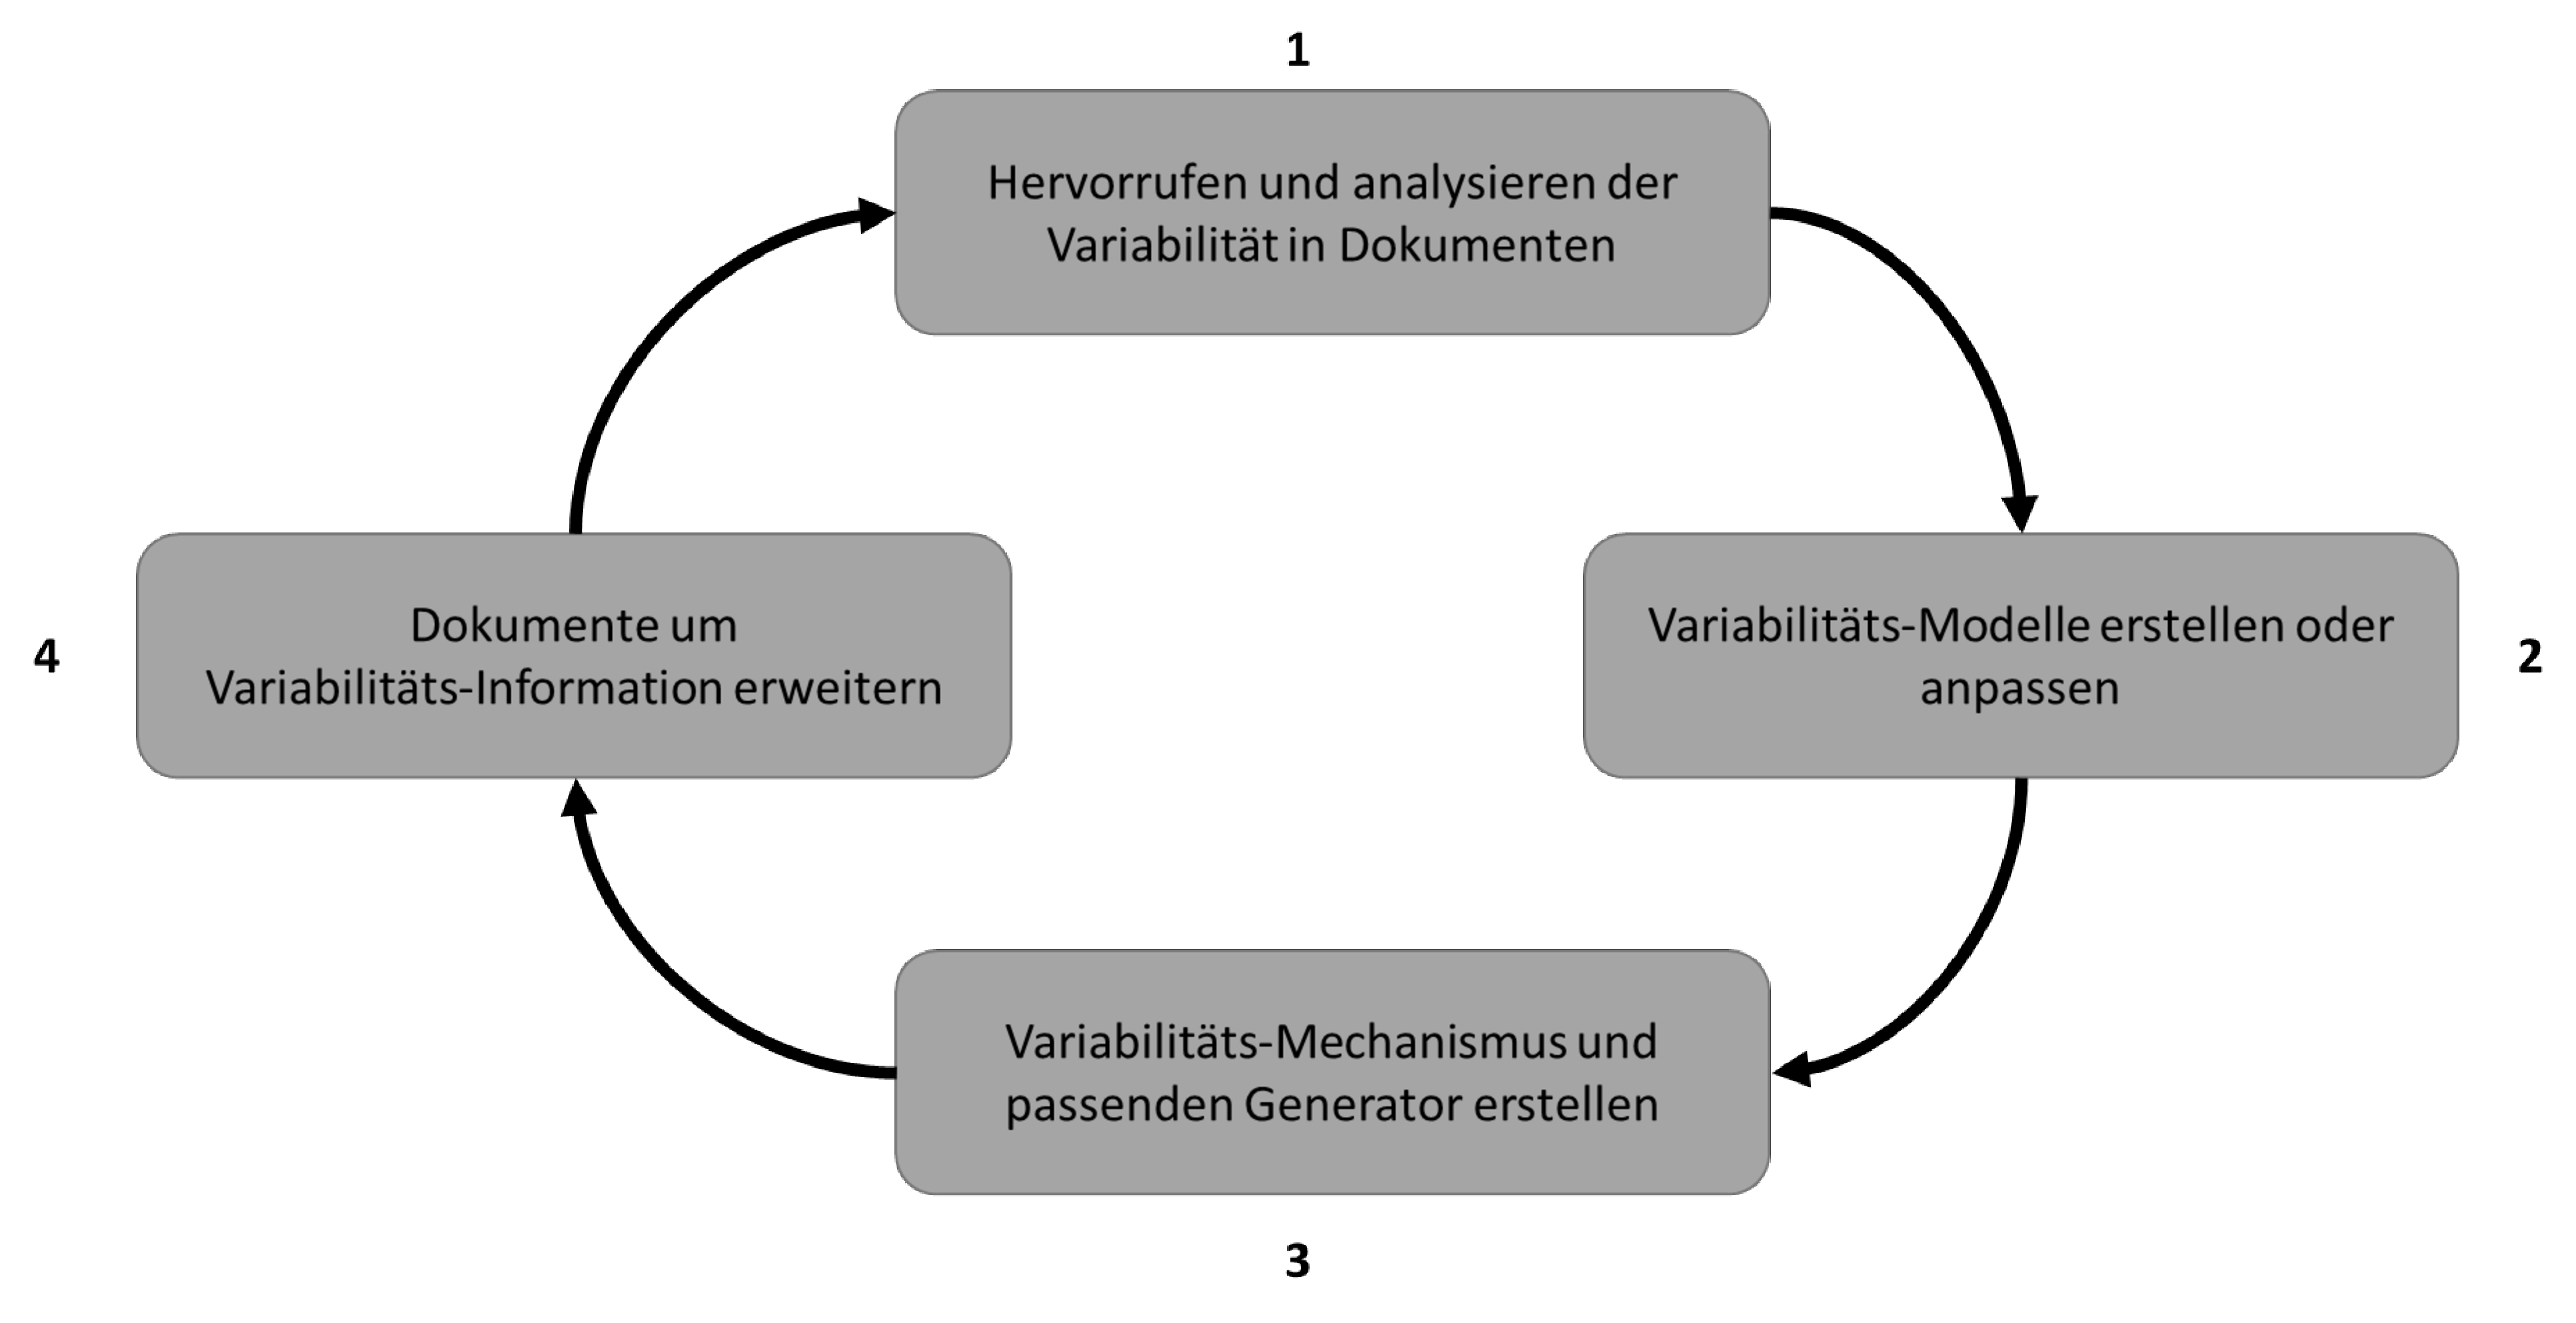
\includegraphics[width=1\textwidth]{img/dopler-approach.pdf}
  \caption{Die vier iterativ zu durchlaufenden Phasen des Dopler
  Ansatzes}
  \label{dopler-approach}
\end{figure}

%% ===========================

Die Tool-Suite enth�lt ein Variabilit�ts-Modellierungs-Tool, einen
Konfigurations-Wizard und \ldots.
	
\begin{figure}[htb]
  \centering
  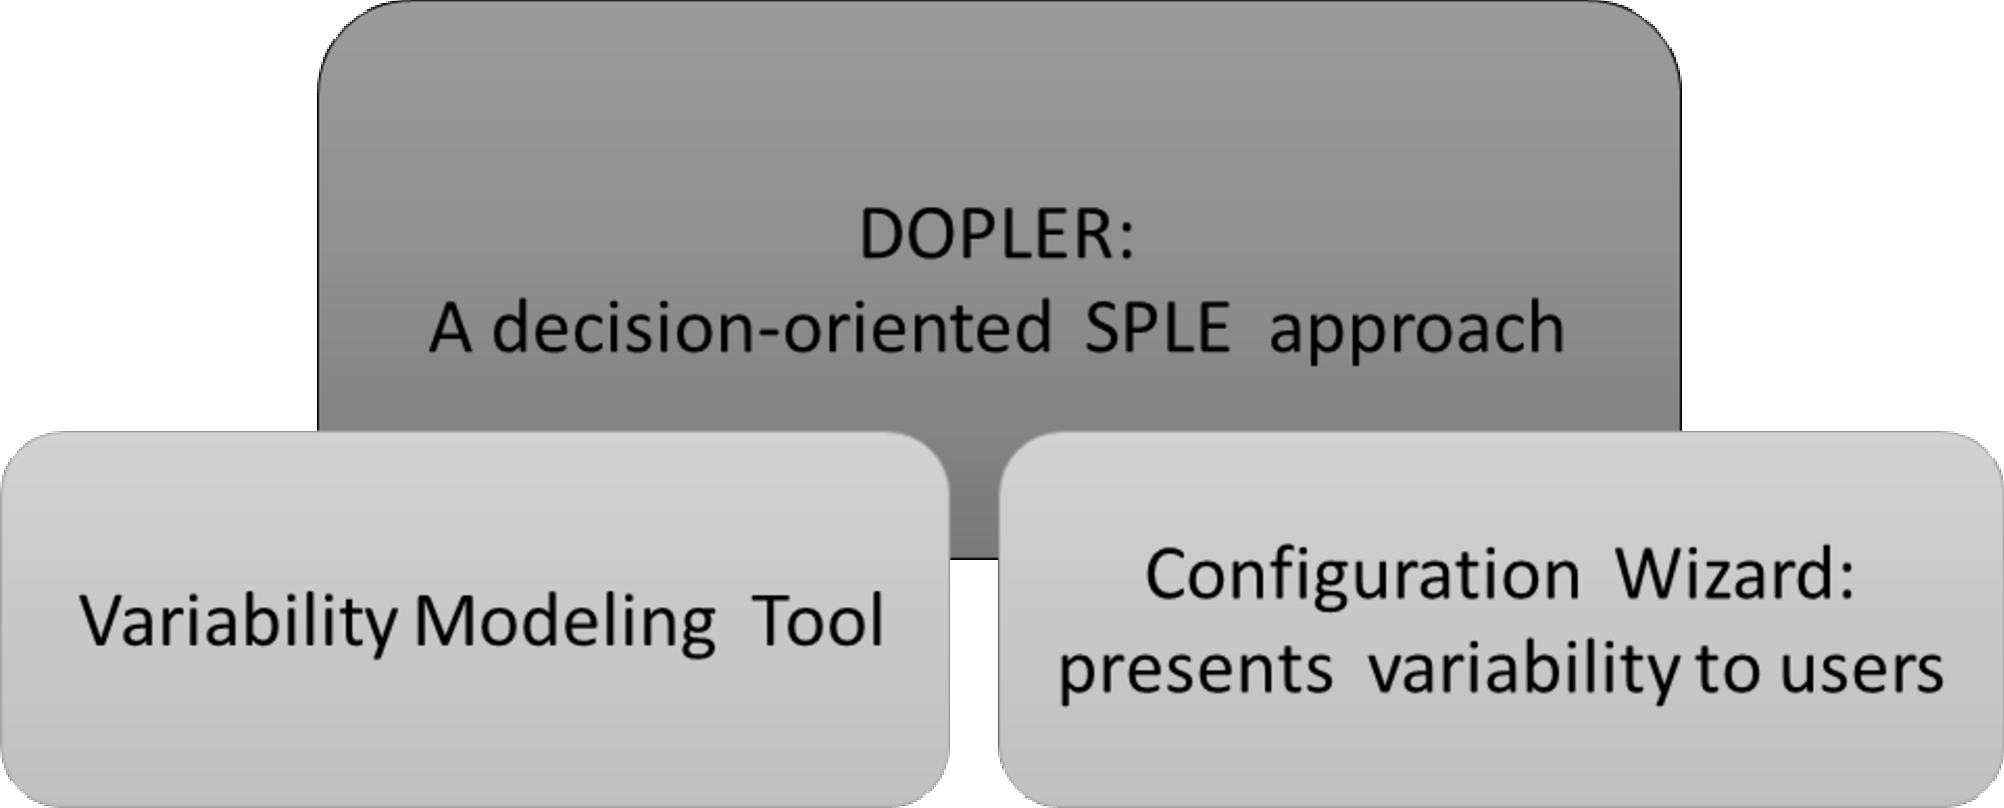
\includegraphics[width=0.4\textwidth]{img/dopler-overview.pdf}
  \caption{Komponenten der \dopler Tool-Suite nach
  \cite{Rabiser}}
  \label{dopler-overview}
\end{figure}

\ref{dopler-overview} muss noch Erweitert werden um die
DecisionKing \& co.
	
Die Decision(Entscheidung) modelliert die Entscheidungspunkte. Sie
enth�lt eine eindeutige Identifikationsnummer, eine Frage und einen
Typen(\ref{fig:dopler-decision-me}. Die Frage wird dem Nutzer bei der
Konfiguration gestellt und die Antwort auf die Frage bestimmt die Zusammensetzung des Dokumentes. Eine Entscheidung
kann von anderen Entscheidungen in zwei Arten abh�ngig sein, siehe
\ref{fig:dopler-meta_model-me}.
Eine hierarhische abh�ngigkeit bedeutet, dass Entscheidungen in einer bestimmten Rheienfolge
gemacht werden m�ssen. Wenn eine logische Abh�ngigkeit besteht dann �ndert eine
Entscheidung die Antworten der davon abh�ngigen.

\begin{figure}[!htb]
  \centering
  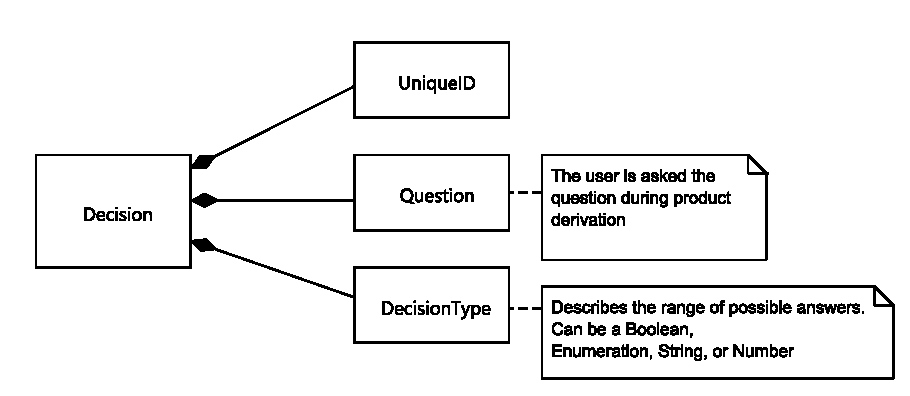
\includegraphics[width=0.9\textwidth]{img/dopler-decision_model-me.pdf}
  \caption{Die Entscheidung und ihre Hauptbestandteile}
  \label{fig:dopler-decision-me}
\end{figure}

Das Dopler-Meta-Model in \ref{fig:dopler-meta_model-me} zeigt auch den
Zusammenhang zwischen den Decisions und Assets. Die Inklusion eines Asset
in das abgeleitete Produkt geschieht durch seine Verbindung zu der Decision.
Die Attribute eine Asset k�nnen von den Antworten auf die Decision Frage beinflusst werden.

\begin{figure}[!htb]
  \centering
  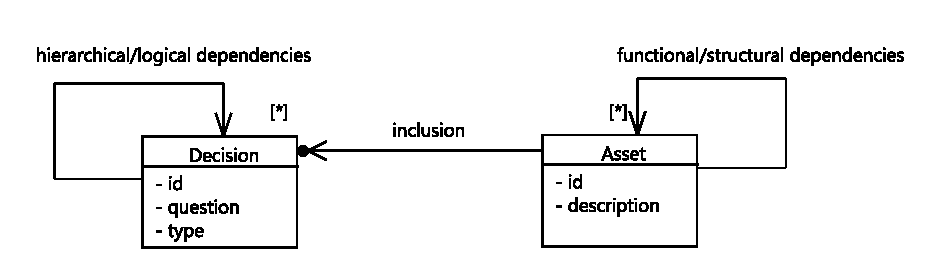
\includegraphics[width=1\textwidth]{img/dopler-meta_model-me.pdf}
  \caption{Dopler Meta-Model aus \cite{Rabiser}.}
  \label{fig:dopler-meta_model-me}
\end{figure}

Das Diagramm \ref{dopler-meta_model} beschreiben.

\begin{figure}[!htb]
  \centering
  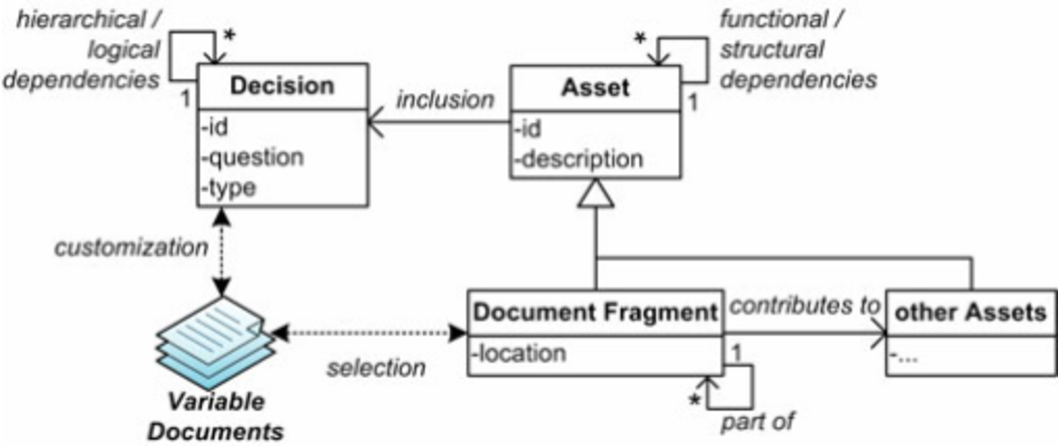
\includegraphics[width=0.8\textwidth]{img/dopler-meta_model.pdf}
  \caption{Dopler Meta-Model mit Dokumenten aus \cite{Rabiser}.}
  \label{dopler-meta_model}
\end{figure}

%% ===========================
\section{Intelligente Augmented-Reality-Handb�cher}
\label{ch:Content8:sec:Section1}
%% ===========================

Der Augmented-Reality-Forschungsbereich des DFKI  arbeitet an der Entwicklung
und Verbesserung von Augmented-Reality-Handb�chern um sie eines Tages in reelen
Szenarien einsetzen zu k�nnen. Ein Augmented-Reality-Handbuch ist ein digitales
Handbuch, dass Schritt f�r Schritt Anleitungen auf einem Head-Mounted-Display
(HUD) auf das Blickfeld des Benutzers projeziert. Jeder Schritt wird dem
Benutzer vorgezeigt bis dieser erfolgreich durchgef�rhrt wurde.

Wenn der Nutzer eine Aufgabe mit Hilfe des Systems durchf�hrt, \ref{fig:test1},
werden zuerst die Schritte notwendigen Schritte f�r die Teilaufgabe
eingebledet, \ref{fig:test2}.
Nachdem der Nutzer mit der Ausf�hrung der Teilaufgabe anf�ngt wird
auf das Sichtfeld der Status der Durchf�hrung mit Hilfe einer Farbkodierung
angezeigt.Dabei bedeutet in \ref{fig:test3} die gr�ne kodierung eine korrekte durchf�hrung.

Eine integrierte Kamera erkennt die Handgriffe und �berlagert diese zusammen mit
einem vorher aufgenommenen Video auf dem HUD um den n�chsten Schritt anzuzeigen.
Der Ansatz kann die vom Benutzer durchgef�hrten Gesten erkennen und braucht
keine speziellen Markierungen.

Das Authoring-Tool kann unabh�ngig(wovon?) die Video-Sequenz in Einzelteile
teilen 

Die Autoren meinen/behaupten dass \ldots


Das Authoring-Tool zerlegt eine einmal gesehene Sequenz
selbstst�ndig in einzelne, unterscheidbare Handlungsabl�ufe
und kombiniert im Anschluss diese einzelnen Kapitel mit
einem stochastischen �bergangsmodell. Zur Laufzeit kann
eine beobachtete T�tigkeit zeitlich den Kapiteln zugeordnet
werden, genau zum passenden Zeitpunkt werden Hinweise
f�r die nachfolgenden Schritte eingeblendet. Das Verfahren
erzeugt vollautomatisch entsprechende �berlagerungen,
indem es ein "Schattenbild" der anstehenden Handlungen
halbtransparent einblendet. Wichtige Details oder zus�tzliche
Hinweise k�nnen durch einfaches Hineinzeichnen grafischer
Symbole wie Pfeile oder Striche verdeutlicht werden.

%Second Sighted glasses erw�hnen
%Ex-Valve Brille

\begin{figure}
\centering
\begin{minipage}{.30\textwidth}
  \centering
  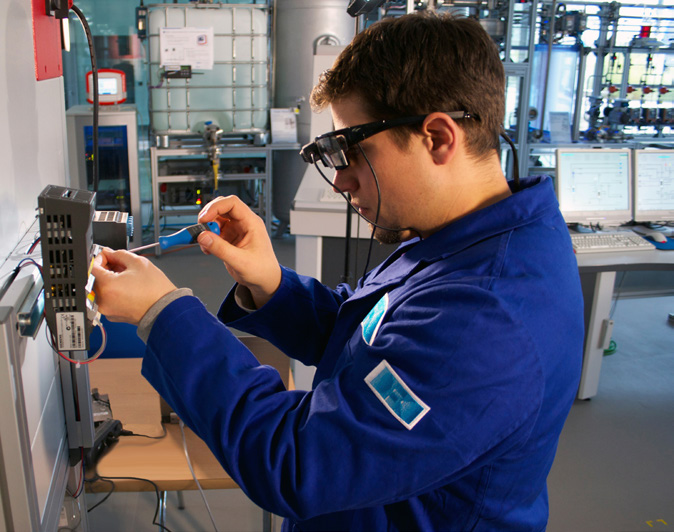
\includegraphics[width=0.9\linewidth]{img/ar-handbook-outside_view.jpg}
  %\captionof{figure}{Der Nutzer f�rht eine Aufgabe mit Hilfe des Systems aus}
  \captionof{figure}{Anwender}
  \label{fig:test1}
\end{minipage}%
\begin{minipage}{.30\textwidth}
  \centering
  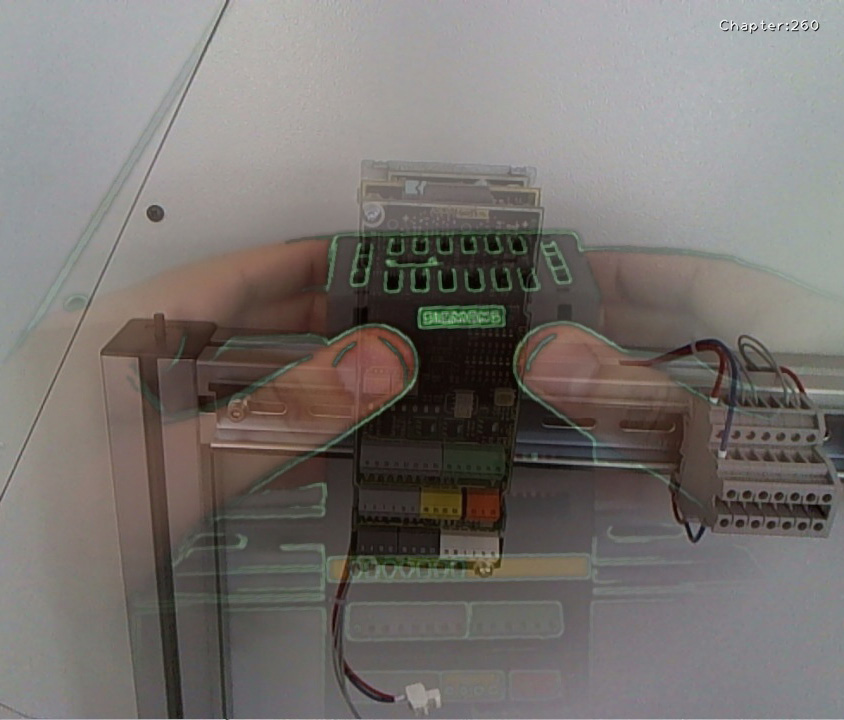
\includegraphics[width=0.9\linewidth]{img/ar-handbook-overlay_bsp.jpg}
  %\captionof{figure}{Die Schritte die durchzuf�hren sind werden im Sichtfeld
  \captionof{figure}{Einblenden der Schritte}
  \label{fig:test2}
\end{minipage}
\begin{minipage}{.30\textwidth}
  \centering
  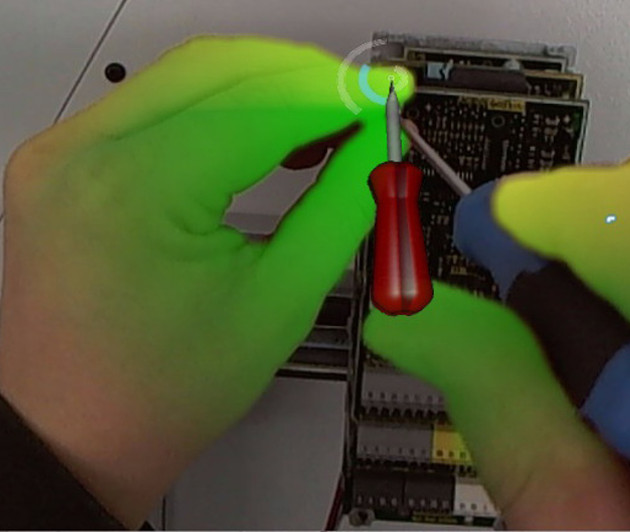
\includegraphics[width=0.9\linewidth]{img/ar-handbook-glove_green.jpg}
  \captionof{figure}{Richtige Durchf�hrung}
 % \captionof{figure}{Die gr�ne F�rbung symbolisiert die richtige Durchf�hrung der Aufgabe}
  \label{fig:test3}
\end{minipage}
% source : http://av.dfki.de/projects_recent/ar-handbook
\end{figure}

%% ==============
\section{Usability of User Interfaces Generated with a Model-Driven
Architecture Tool}
\label{ch:Existierende}
%% ==============

\ldots

%% ==============
\section{User comprehension performance for dataflow-based rules in smart
Environments}
\label{ch:Existierende}
%% ==============


%% ==============
\chapter{Leichtgewichtige Generierung(Meine Idee)}
\label{ch:MeineIdee}
%% ==============

\dots

%% ==============
\chapter{Vergleich der Ans�tze}
\label{ch:Vergleich}
%% ==============

\begin{table}
  %\rowcolors{3}{green!25}{yellow!50}
  \caption{Vergleich der Ans�tze(unter dem Aspekt der Benutzbarkeit)}
  \centering
  \begin{tabular}{l c c c c c}
    %heading
    \hline\hline
    
    & \dopler & AR-Handbook & Modellgetriebene GUI & Regelbasiert &
    Meine Idee
    \\
    [1ex]

    \hline
    %heading end
    
    %     DUdu & &&& \parbox[t]{5cm}{Sales and marketing
    %     people \\ porduct managers} \\ [1ex]
    
    Ansatz &  Entscheidungs orientiert\\ [1ex] 
    
    Interaktionsmodus \\ [1ex]
    
    Quell-Artefakte \\ [1ex] 
    
    Generierte Artefakte & Fertige Dokumente & \\ [1ex] 
    
    End-Nutzer & Vertrieb, Marketing, & \\
    & Produkt-Management &&&& \\ [1ex]
    
    Form der Unterst�tzung & Textuell & Graphisch, VR & Graphisch &&
    \\ [1ex]
     
    Flexibilit�t \\ [1ex] 
    
    Dom�nenexperten & \textsc{Ja} & \textsc{Ja} & \textsc{Nein} &
    \textsc{Ja} & \textsc{Nein} \\ [1ex]
    
    Wiederverwendung \\ [1ex]
    
    Aufwand f�r die Instandsetzung \\ [1ex]
    
    Aufwand f�r die Benutzung \\ [1ex]
    
    Genauigkeit der Beschreibung \\ [1ex]
    
    Synchronisierungsaufwand \\ [1ex]
    
    Aufwand f�r die Erstellung neuer Handb�cher \\ [1ex] 
    
    Anwendungsszenarien & & physiche Umgebung\\ [1ex]
    \hline
  \end{tabular}
  \label{table:tab1}
\end{table}

Eine �bersicht der Ans�tze findet man in den Tabellen
\ref{table:tab1} und \ref{table:tab1}.

Genauigkeit der Beschreibung: kann das Garantiert werden wenn menschen das
System intepretieren?


%==============================================
%% ==============
\chapter{Weiteres Vorgehen}
\label{ch:NextSteps}
%% ==============

Usability studies machen
Am anfang um eine Hypothese zu erstellen und sehen was leute von so einem System
erwarten

 !System definieren!
 
Punkte finden die interessant sind/interessant zu beschreiben sind.
Formative studie - ?
Qualitativ, qunatitative?

Interviews erstellen -> Requirements sammeln -> Hypothese

Studien erstellen um zu sehen ob eine statistisch signifikanter Unterschied
zwischen den statisch erstellten und den dynamisch generierten besteht.

Wizard of Oz studie => Referenzimplementierung machen

Idee:
	Seite erstellen die einen konfigurator darstellt. User konfigurieren lassen.
	Nach einiger zeit den usern das ding in die Hand dr�cken und arbeten lassen.
	
2x5/7 Leute sollte man haben f�r eine Usability studie
Gruppen Interviews sind nicht schlecht um Gruppendynamik zu f�rdern.
Tutorium Users study?

Methodik muss fest sitzen! 


%% % ===========================
\section{Dokumentengenerierung in industriellen Umgebungen}
\label{sec:documentGeneration}
% % ===========================

Um die Generierung von Dokumenten als auch von Softwaresystemen aus
demselben Variabilit�tsmodel zu erlauben, wurde der in \cite{Rabiser2010}
beschriebene Ansatz entwickelt.
Grundlegend bei der Erstellung des Ansatzes war die Beobachtung, dass viele
Entscheidungen die w�hrend der Ableitungsphase des Produktes gemacht werden,
sowohl f�r die Dokumentation als auch f�r das Softwaresystem relevant sind.
Der Ansatz wurde, mit Hilfe der \dopler Werkzeuge \cite{Dhungana2007,
Dhungana2010}, Erfolgreich auf zwei Produktlinien mit verschiedenen Reifegraden
angewandt. Bei der ersten Produktlinie handelt es sich um eine Anwendung zur
Prozessautomatisierung von Siemens VAI, dessen technische Variabilit�t schon
modelliert war und technische Dokumentation erstellt werden sollte. Die zweite
Anwendung verlief bei der Siemens AG und es mussten ohne ein schon vorhandenes
Variabilit�tsmodell kundenspezifische Verkaufsdokumente erstellt werden.

% =======
\subsection{Flexibler Ansatz zur Dokumentengenerierung}
\label{sec:doplerSchritte}
% =======

Der in \cite{Rabiser2010} beschriebene Ansatz kann laut den Autoren unabh�ngig
vom Reifegrad, der Modellierungstechnik der Variabilit�t oder der zu
generierenden Dokumenttypen verwendet werden. Vier Grundlegende Schritte sind
iterativ durchzuf�hren (siehe auch Abbildung \ref{fig:dopler-approach}):

\begin{enumerate}
  \item Extrahieren und Analysieren der Dom�nenvariabilit�t
  
  \item Variabilit�ts-Modelle erstellen oder anpassen
  
  \item Variabilit�ts-Mechanismus und passenden Generator erstellen
  
  \item Dokumente um Variabilit�ts-Information erweitern
  
\end{enumerate}

Durch die Extraktion der Dom�nenvariabilit�t durch Produktlinienexperten und
Dom�nenexperten des Produkt-Managements oder des Vertriebs kann der wesentliche
Teil der existierenden Variablit�t identifiziert werden. Mit den so gewonnenen
Informationen ist es m�glich, Variabilit�tsmodelle zu erstellen oder anzupassen.
Die gew�hlte Modellierungstechnik sollte flexibel sein und fortgeschrittene
Automatisierung w�hrend der Produktableitung zulassen. Um
Variabilit�tsinformation in den Dokumenten abzulegen ben�tigt man einen
Mechanismus, wie zum Beispiel ein strukturiertes Dokumentenformat mit
einer XML basierten Markupsprache (DocBook). Diese Informationen werden von
einem Generator benutzt, um die produktspezifischen Dokumente zu erstellen.
  

\begin{figure}[htb]
  \centering 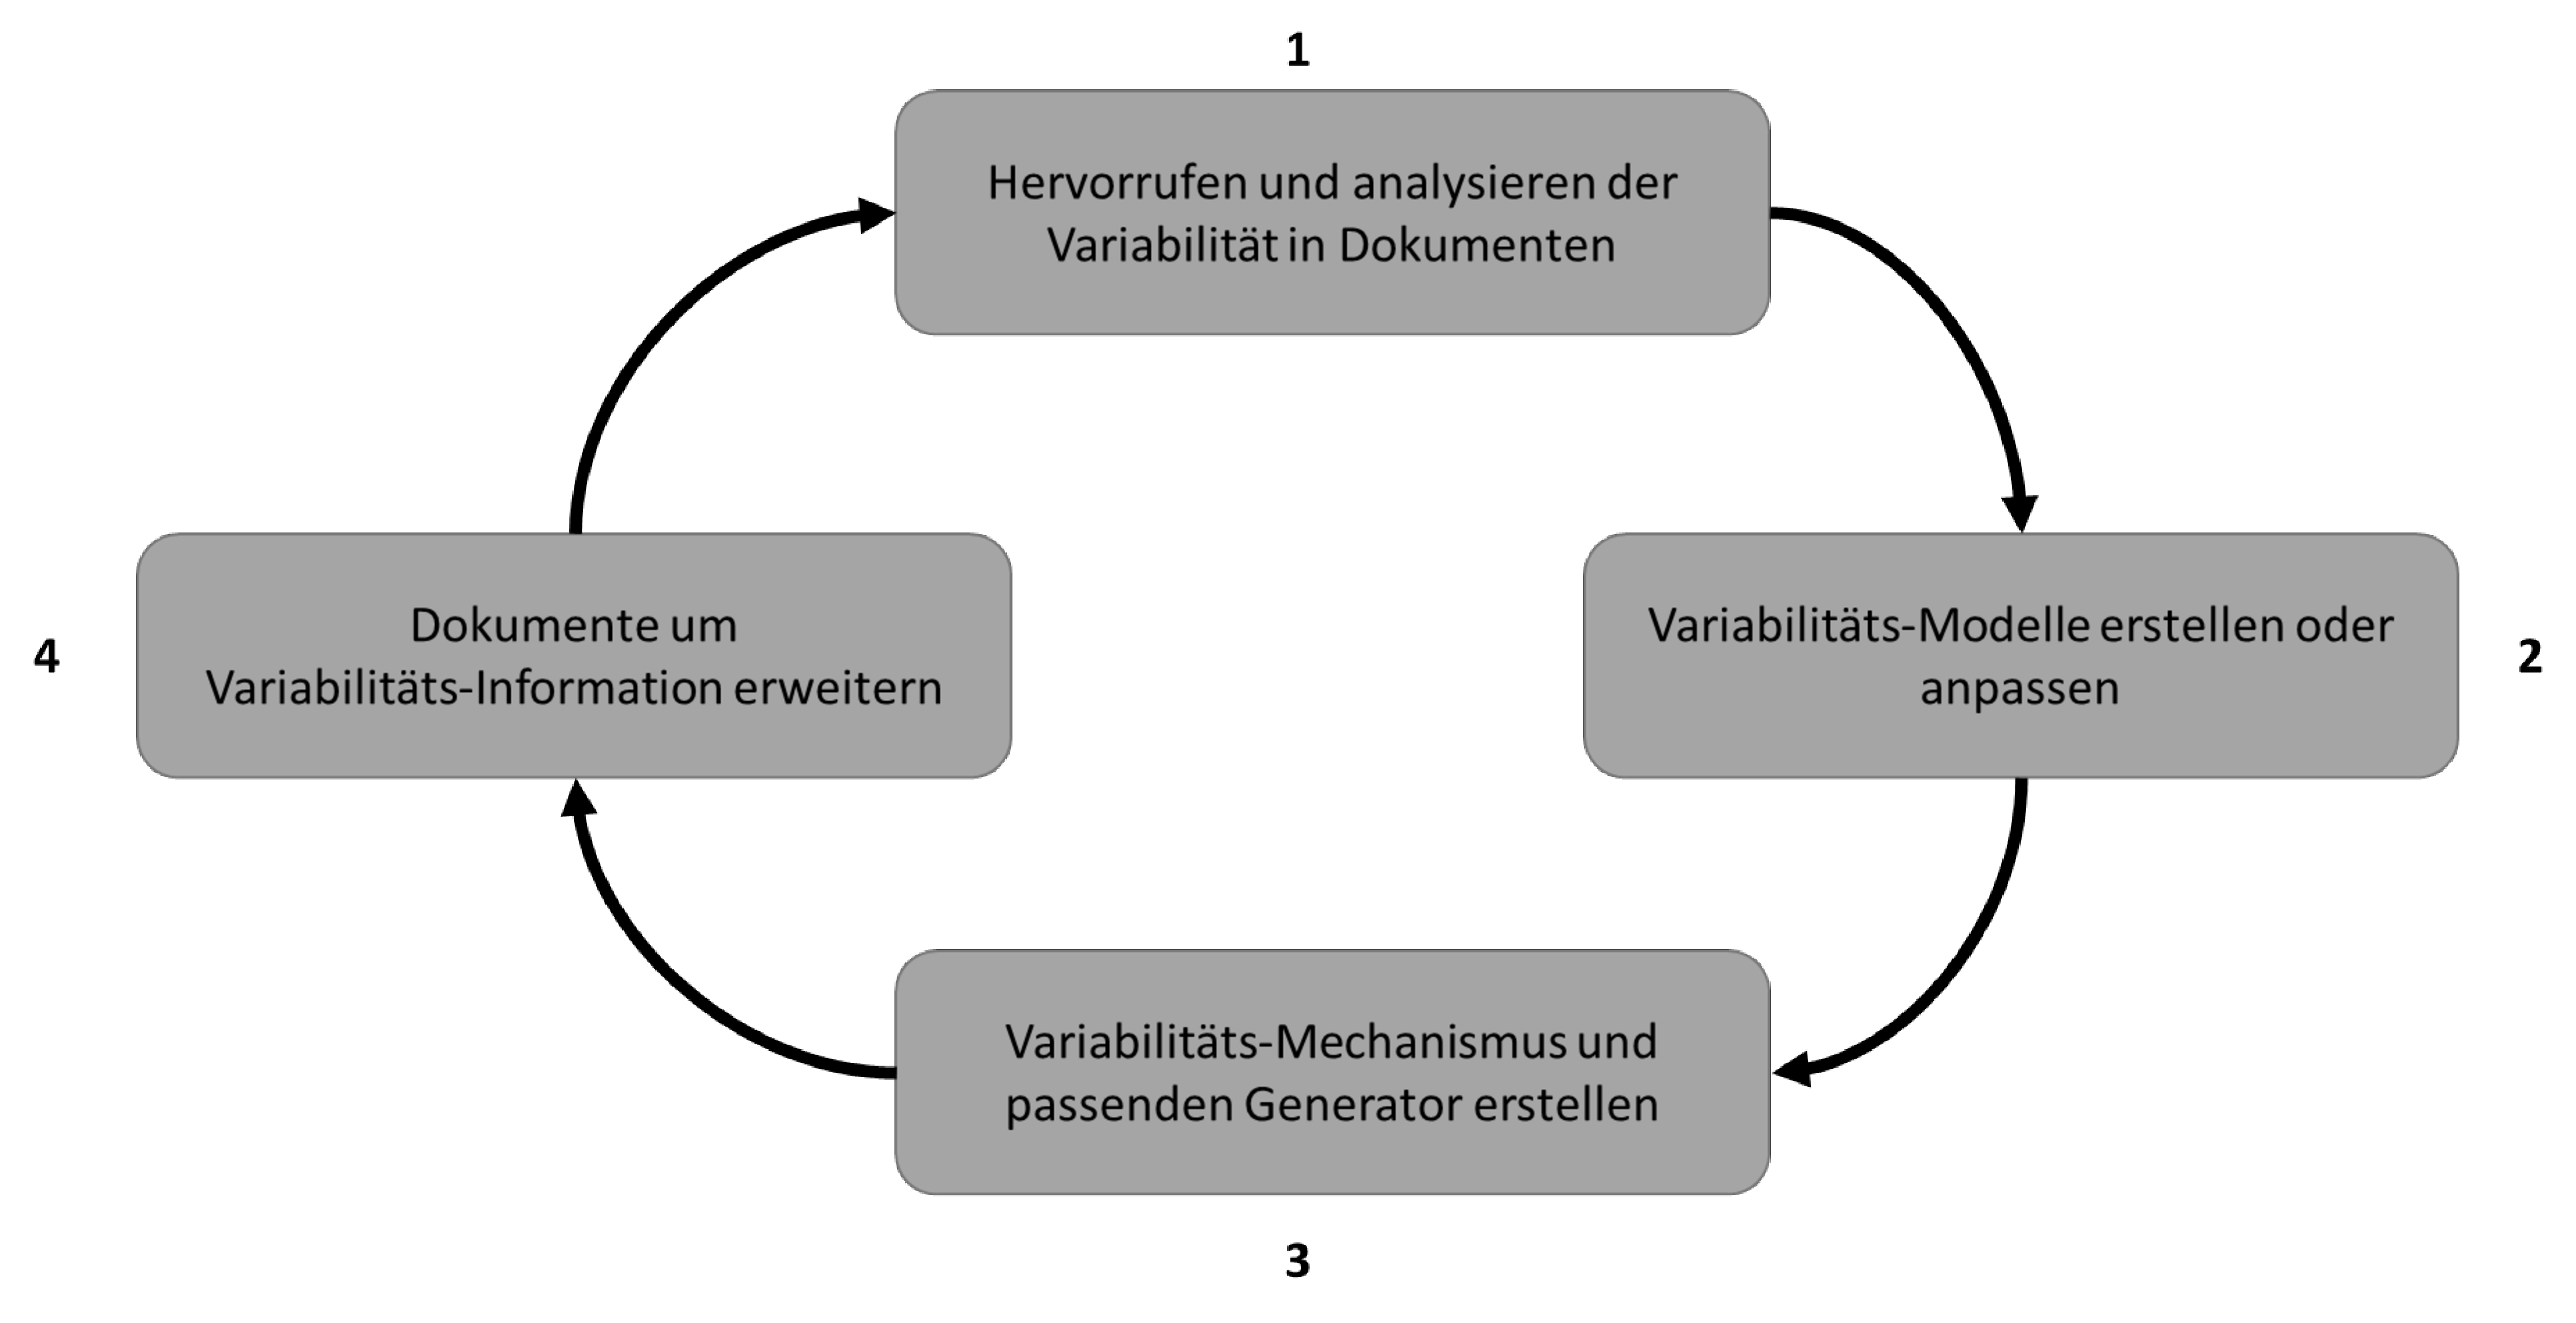
\includegraphics[width=0.9\textwidth]{img/dopler-approach.pdf}
  \caption{Die vier iterativ zu durchlaufenden Phasen des Ansatzes zur
  Dokumentengenerierung aus \cite{Rabiser2010}. Variationspunkte und Varianten
  werden in Schritt (1) von Dom�nenexperten hervorgehoben und in Beziehung mit
  den Modellen aus Schritt (2) gestellt. Die Beziehungen werden mit Hilfe des
  Mechanismus aus Schritt (3) realisiert. Der letzte Schritt (4) webt die
  Informationen in die Dokumente ein.}
  \label{fig:dopler-approach}
\end{figure}

% =======
\subsection{\dopler Metamodell}
% =======

Auf Ebene der Variabilit�tsmodellierung werden zwei Grundlegende Entit�ten
definiert: Assets und Decisions (vgl. Abbildung \ref{fig:dopler-meta_model}).
Die \dopler Werkzeuge erlauben es, durch dom�nenspezifische Metamodelle, deren
Elemente von den Grundentit�ten \emph{Asset} und \emph{Decision} erben, Dom�nen
mit beliebiger Granularit�t und Abh�ngigkeiten zu modellieren. Assets sind die
Artefakte der Produktlinie (Dokumente oder Technische Bestandteile). Decisions
hingegen sind die Entscheidungsbasis, anhand derer die Konfiguration der Assets
stattfindet. Diese sind analog zu den in der Variabilit�tsmodellierung
eingesetzten Entscheidungspunkten (Variation Points).
Die Funktionsabh�ngigkeit und der strukturelle Aufbau des Systems k�nnen durch
die im Metamodell vorhandene Abh�ngigkeitsbeziehung zwischen Assets modelliert
werden. Logische und hierarchische Zusammenh�nge zwischen den zu treffenden
Entscheidungen (Decisions) werden im Metamodell ber�cksichtigt und erlauben die
Definition von Reihenfolge- und Verhaltensbeziehungen.

%=======
\begin{figure}[htb]
  \centering
  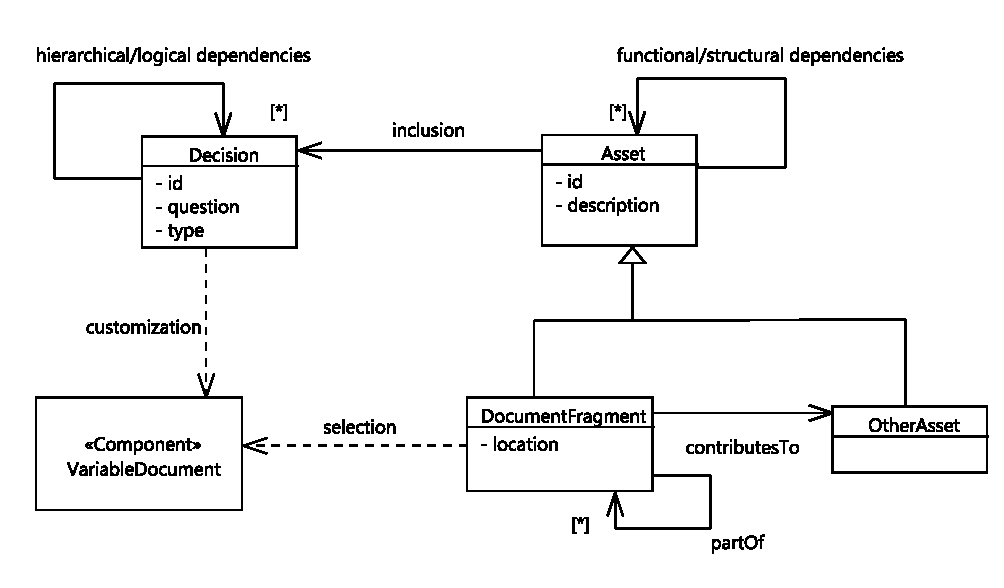
\includegraphics[width=0.8\textwidth]{img/dopler-meta_model_complete-me.pdf}
  \caption{\dopler\ Meta-Model mit Dokumenten aus \cite{Rabiser2010}.}
  \label{fig:dopler-meta_model}
\end{figure}
%=======

Die Inklusion eines Asset in das abgeleitete Produkt geschieht durch seine
Verbindung zu der Decision. Auch die Attribute eines Asset k�nnen von den
Antworten auf die Frage der Decision beinflusst werden. Die wesentlichen
Elemente einer Decision sind die Frage und der Typ. Die Frage wird dem Nutzer
bei der Konfiguration gestellt und dessen Antwort bestimmt die Zusammensetzung
des Dokumentes, wobei der Typ das weitere Vorgehen bestimmt. Bei dem Typen der
Decision werden von bin�ren Antworttypen (Ja/Nein Antworten) bis hin zu
komplexer Logik darstellende Datentypen verwendet ([Beispiel ??]).

\dopler erlaubt es dom�nenspezifische Assets zu definieren, indem ein vom
\dopler Metamodell erbendendes Modell einer spezifischen Organisation oder
Kontextes erstellt wird. Um Dokumente zu generieren kann man Teile oder sogar
ganze Dokumente als Assets in den Modellen repr�sentieren. So wurden, wie in
Abbildung \ref{fig:dopler-meta_model}, die Assets erweitert in dem das
\emph{DocumentFragment} eingef�hrt wurde. Dieses kann Teile eines Dokumentes wie
Kapitel oder Abschnitte repr�sentieren. Um auch den Fall zu modellieren, dass
bestimmte Fragmente Teil von anderen Fragmenten sind, wurde in dem abgebildeten
Modell eine Aggregation zwischen den Dokumentfragmenten eingef�hrt.

Spezifisch f�r die Erstellung von Dokumenten k�nnen Dokumentfragmente als
Dom�nenelemente modelliert werden, die von der Grundentit�t Asset erben. So kann
dieselbe Decision benutzt werden um mehrere Dokumentfragmente zu verwalten.
Dokumentfragmente und Komponenten des Systems k�nnen dadurch einheitlich
behandelt werden. Dokumentfragmente erlauben die Modellierung der grobk�rnigen
Variabilit�t. Feink�rnige Anpassungen werden durch einen spezifischen
Variabilit�tsmechanismus realisiert.

% =======
\subsection{Dokumentstruktur und ihren Einfluss auf die Generierung}
% =======

Der Profil-Mechanismus des DocBook-Standards wird in der Arbeit benutzt um
Elemente und Attribute zu implementieren, die die Variationspunkte in den
Dokumenten definieren. Die zentrale Erweiterung zu DocBook ist das
\emph{doplerdoc} Attribut. Es koppelt das Markup-Element an ein Dokumentfragment
und erlaubt es so optionale oder alternative Texte zu definieren. Durch diesen
Mechanismus sind auch Querverweise m�glich und Platzhalter k�nnen in Verbindung
mit dem \emph{doplerdocplaceholder} Element erstellt werden.

In Listing \ref{lst:dopler_docbook_xml} wird ein Beispiel aus einem
DocBook-Dokument mit der \dopler Erweiterung aufgef�hrt. Das Kapitel
\emph{cooling} wird in die Dokumentation nur aufgenommen, wenn das
Dokumentfragment \emph{cooling\_chapter} aufgrund einer Decision
aufgenommen wurde.

% =======
\lstset{breaklines=true,language=XML,caption={Das Element
\emph{doplerdocplaceholder} mit dem \emph{doplerdoc} Attribut dient als
Platzhalter f�r den K�hlungsmechanismus \emph{cooling\_mech}
\cite{Rabiser2010}},label=lst:dopler_docbook_xml}
\lstinputlisting[language=XML]{listings/docbook_example.xml}
% =======

Die Werkzeugkette, die die Autoren in den in \cite{Rabiser2007} durchgef�hrten
Studien eingesetzt haben, besteht aus verschiedenen Auspr�gungen des \dopler
Werkzeugs.
Als Generator wurde eine f�r jede Dom�ne angepasste Erweiterung des \dopler
Konfigurationswerkzeugs erstellt. Ein Variabilit�ts-Modellierungs-Tool und ein
Konfigurations-Wizard, um den Nutzer durch Produktableitung zu f�hren, sind Teil
der Werkzeugkette.

Der Ablauf zur Generierung von Dokumenten beginnt mit der Erstellung eines
Variabilit�tsmodells. Die Antworten auf die Fragen der Decisions werden durch
den Nutzer mit Hilfe eines Konfigurationsassitenten (z.B. \dopler
Konfigurations-Wizard) in das Modell eingetragen. Das variable Dokument, das
zentrale Artefakt im Prozess der Dokumentengenerierung, entsteht durch das
Erweitern existierender Dokumentatino mit der im Variabilit�tsmodell
existierenden Variabilit�tsinformation und eine st�ndige R�ckkopplung zu dem
Variabilit�tsmodell.

% =======
\begin{figure}[htb]
  \centering
  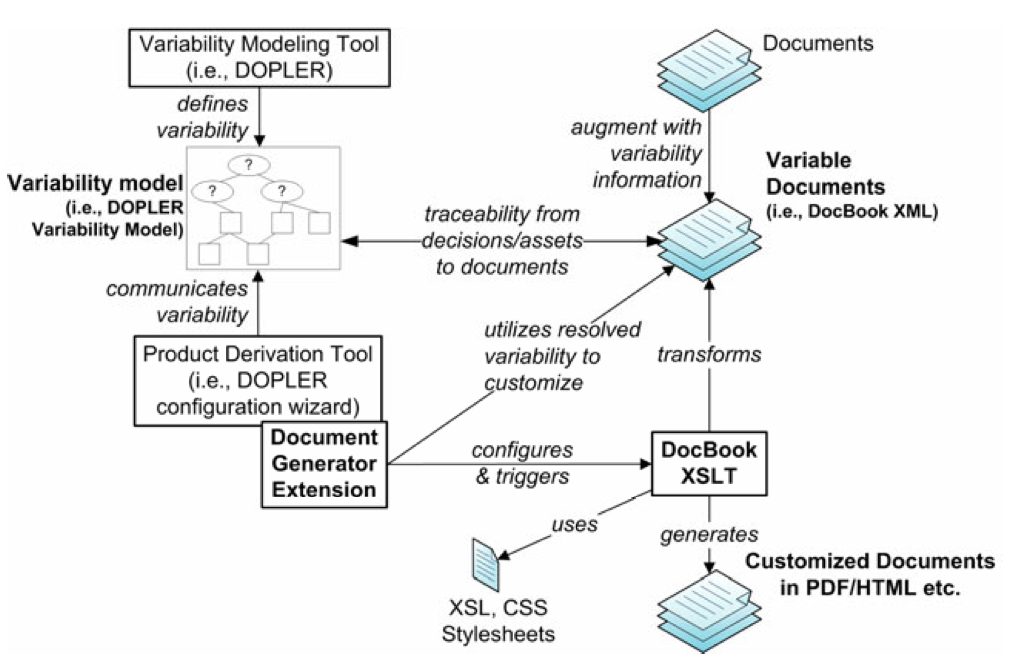
\includegraphics[width=0.8\textwidth]{img/dopler-document_generation.png}
  \caption{\dopler �berblick �ber den Generierungsprozess der finalen
  Dokumentation aus dem Variabilit�tsmodell in
  \cite{Rabiser2010}.}
  \label{fig:dopler-meta_model}
\end{figure}
% =======

Der Dokumentengenerator kann mit Hilfe der durch den Nutzer aufgel�sten
Variabilit�t die Anpassung des variablen Dokuments durchf�hren und weist die
DocBook-XSLT-Engine an ein Dokument im gew�nschten Ausgabeformat (z.B. PDF) zu
erstellen. Die variablen Dokumente werden mittels der DocBook-Engine in ein
Ausgabeformat (z.B. PDF) transformiert und mit Hilfe von formatiert.
Formattierungsoptionen sind mit XSL oder CSS realisierbar und k�nnen auch durch
Decisions konfiguriert werden.

% =======
\subsection{Ergebnisse industrieller Studien}
% =======

Die gewonnenen Erkenntnisse aus den zwei industriellen Anwendungen des Ansatzes
werden im weiteren beschrieben.

Im ersten Anwendungsfall, bei der Siemens VAI, waren Teile der Dokumentation f�r
Benutzer schon als DocBook-Quellen vorhanden. Des weiteren waren die
Variabilit�tsmodelle schon vorhanden und die automatische Generierung von
Produktkonfigurationen wurde bereits unterst�tzt.  In der ersten Phase der
Methode, das Extrahieren und Analysieren der Dom�nenvariabilit�t (vgl. Kapitel
\ref{sec:doplerSchritte}) wurden folgende Kategorien von Variabilit�t, die laut
einer Befragung der Dom�nenexperten am meisten auftreten,
in Betracht genommen:

\begin{itemize}
  \item Optionale Teile der Dokumentation
  \item Querverweise und deren Konsistenz
  \item Platzhalter (z.B Name des Kunden)
  \item Grammatikalische Variation (Pluralbildung)
  \item Multi-Media-Objekte (z.B. Bilder)
  \item Formatierung und Layout (durch XSL oder CSS Style-Sheets
  realisierbar)
\end{itemize}

Bei der Erstellung der Variabilit�tsmodelle konnten 70\% der Decisions aus den
technischen Variabilit�smodellen benutzt werden. In den restlichen F�llen wurden
Decisions spezifisch f�r die Dokumentengenerierung erstellt. Ein Generator wurde
so erstellt, dass er die technische Benutzerdokumentation laut den Decisions
aufbauen kann. Die Aufgabe der Erweiterung der Dokumente mit der
Variabilit�tsinformation (der 4. Schritt der Methode) konnte erfolgreich von den
Dom�nenexperten durchgef�hrt werden, nachdem f�r jede oben erw�hnte Art von
Variabilit�t ein Beispiel zur Verf�gung gestellt wurde.

Die mit dem Ansatz erstellte und durch die \dopler Tools Realisierte
Werkzeugkette unterst�tzt sowohl die Variabilit�tsmodellierung der Software als
auch der Dokumente. Ein einziges Entscheidungsmodell wird benutzt um die
Produktkonfiguration als auch die Technische Benutzerdokumentation zu erstellen.
F�r den Fall, dass Kunden eigene Erweiterungen f�r das System entwickeln wollen,
m�ssen sehr spezifische Dokumente geliefert werden. Diese waren vor der
Einf�hrung der \dopler Werkzeuge nicht realisierbar.

In der zweiten Industriellen Anwendung, bei der Siemens AG, mussten
kundenspezifische Verkaufsdokumenete erstellt werden, wobei es keine existierende
Variabilit�tsmodellierung gab. Zu den oben erw�hnten Variabilit�tspunkten kamen
noch variantenabh�ngige Berechnungen der Preise und anderer Indikatoren hinzu.
Au�erdem gab es in diesem Fall mehr Alternativtexte und einige Variationspunkte
die einen dokumenten�bergreifenden Einfluss hatten.

Der in \cite{Rabiser2010} beschriebene Ansatz erlaubt es an den Entwicklungs und
Generierungsprozesses von Software die Generierung von Dokumenten einzubinden.
Die Auswechselbarkeit der Werkzeuge zur Variabilit�tsmodellierung und
Generierung erlauben eine gro�e Flexibilit�t bei der Anwendung auf verschiedene
Dom�nen und unterschiedliche technische Gegebenheiten. Besonders
nicht-technisches Personal wird durch die so entstandene Werkzeugkette in der
Generierung von spezifischen Dokumenten unterst�tzt.

%Die beschreibung der Systemmodelle wird nicht erl�utert - vielleicht in anderen
%Papern? - Paper zu Eclipse
% %% ==============
\chapter{Leichtgewichtige Generierung mit InstaGuide}
\label{ch:Instaguide}
%% ==============

Die vorl�ufigen Resultate der AR-Ans�tze bieten eine vielversprechende
L�sung um die Installation ubiquit�rer Systeme zu erleichtern (vgl.
Kapitel \ref{sec:arhandbook})[Sau mai bine Kapitel Vergleich]. Der in
\ref{sec:documentGeneration} beschriebene Ansatz leidet darunter, dass
Expertenwissen f�r jede Variante ben�tigt wird. Der dort beschriebene
Ansatz dient auch der Generierung schwergewichtiger Dokumente.
Man kann sich aber die Frage stellen ob die Nachteile solcher Ans�tze
behoben, die Vorteile aber beibehalten werden k�nnen.
Eine leichtgewichtige, textuelle Beschreibung die aus das System
beschreibenden Modellen, automatisch generiebar ist, k�nnte L�cken
f�llen. Dazu wird ein Ansatz zur dynamischen Generierung
nat�rlichsprachlicher Anleitungen f�r die Installation von Ger�ten in
Ubiquit�ren Umgebungen pr�sentiert. Modell-zu-Modell-Transformationen
eignen sich gut, um verschiedene Sichten (Modelle) auf ein System
voneinander abzuleiten. Auf Basis einer formalen Funktionsbeschreibung
und des aktuellen Kontextes (z.B. Zusammenh�nge zwischen Ger�ten,
Zustand der Ger�te) soll mittels modellgetriebener Transformationen
automatisiert eine aktuelle, situationsadaptive, deskriptive,
informelle Sicht auf die Benutzung erzeugt werden. Das Modell der
Systembeschreibung dient als Ausgangspunkt der Generierung. Des
weiteren sollte die Variabilit�t des Systems bekannt und in einem
Modell festgehalten sein. Falls dies nicht der Fall ist kann wie in
\cite{Beckmann2004} (vgl. Kapitel \ref{sec:documentGeneration})
vorgegangen werden um diese zu bestimmen.

Die Schritte die in der Implementierung des Ansatzes automatisiert
ablaufen sollen sind folgende (vgl. auch Abbildung
\ref{fig:instaguide-ueberblick}:
\begin{enumerate}

  \item \textbf{Ein filtriertes Modell des Systems erstellen}\\
  Mit Hilfe eine Modelltransformation sollen die f�r das Handbuch
  relevanten Entit�ten aus dem formalen Modell des Systems extrahiert.
  Diese werden in das filtrierte Modell gespeichert. Falls das System
  durch mehrere Modelle beschrieben wird, um verschiedene Sichten
  darauf zu erlauben, kann diese Modelltransformation diese vereinen
  und die relevanten Daten aus allen Modellen extrahieren.
  
  \item \textbf{Ein f�r Handb�cher semantisch reiches Modell
  erstellen}\\
  Das filtrierte Systemmodell wird weiter in ein Modell �berf�hrt, das
  sich f�r die Generierung von nat�rlicher Sprache eignet. In diesem
  Schritt wird ein zweites Modell herangezogen, das mit Hilfe von
  Meta-Informationen �ber das System ausgestattet ist. Diese
  Meta-Informationen k�nnen Satz-Templates, Priorit�ten der
  Komponententypen oder weitere Abh�ngigkeiten enthalten.
  
  \item \textbf{Generierung von nat�rlicher Sprache}\\
  Durch eine weitere Transformation soll aus dem semantisch reichen
  Modell das nat�rlichsprachliche Handbuch generiert werden. Die
  Generierung von nat�rlicher Sprache ist komplex, deshalb wird sich
  dieser Ansatz zuerst auf einfache grammatikalische Konstrukte
  konzentrieren und es wird versucht ohne ein grammatikalisches
  Framework auszukommen.
  
\end{enumerate}

Ontologien wurden in \cite{Eriksson2007} benutzt um textuelle
Dokumente zu erweitern. Die so entstandenen semantischen Dokumente
erlauben es den Benutzern auf mehreren Arten auf das Wissen
zuzugreifen. Der hier beschrieben Ansatz soll auch eine Art der
Wissensrepr�sentation, wie zum Beispiel Ontologien, verwenden um damit
die Modelltransformationen zu erweitern. So k�nnen Meta-Informationen,
die nicht in dem formalen Modell des Systems gespeichert werden
herangezogen werden um ein semantisch reicheres Modell zu erhalten,
das auch die Umsetzung in nat�rlicher Sprache erleichtert.

% ==========
\begin{figure}[htb]
  \centering
  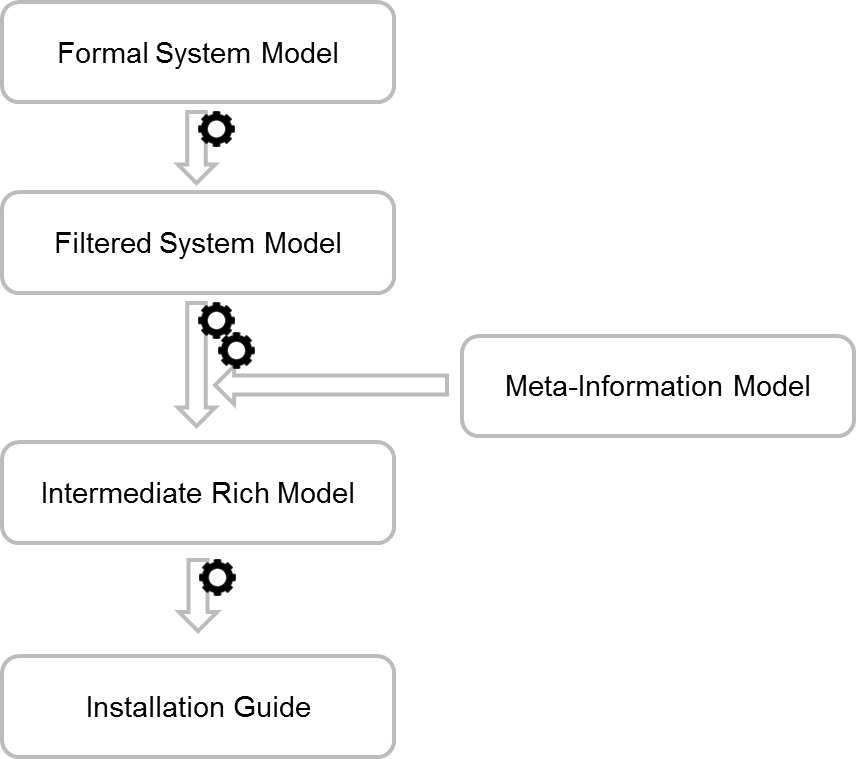
\includegraphics[width=0.8\textwidth]{img/instaguide-overview.png}
  \caption{Instaguide-Ansatz �berblick}
  \label{fig:instaguide-ueberblick}
\end{figure}
% ==========

Ein Vorteil dieses Ansatzes ist der hohe Automatisierungsgrad und die
Unabh�ngigkeit vom Expertenwissen.
Diese Eigenschaften sind gegeben, da die Modelltransformationen
automatisch ablaufen und nach der Erstellung der Dom�nenspezifischen
Modelle kein Expertenwissen in die Generierung der Handb�cher f�r die
unterschiedlichen Varianten der Software einflie�en muss.

Die Herausforderung ist es Transformationen zu erstellen die ein f�r
den Menschen nutzbares Resultat liefern und auch schnell genug laufen
um mit jeder �nderung das Neugenerieren in kurzer Zeit zu erm�glichen.
Studien �ber die Eignung einer solchen L�sung sind notwendig um den
Nutzen und die Effektivit�t der L�sung zu testen.

\texttt{Hier werden noch ein paar St�cke aus dem SWC Antrag
eingepflegt}


Um ein finales Handbuch zu erhalten, dass auch f�r nicht-technische Endnutzer
geignet ist werden die automatisch erstellten Fragmenten in eine vorher
definierte Struktur eingebettet. Diese Struktur kann mittels DocBook definiert
werden und erm�glicht die unabh�ngige Integration von Pr�sentationsteilen der
Marketing Abteilung (Bilder, Adressen etc.) als auch die Einbindung von
legislativ vorgesehenen Plichteintr�gen.

Eine Kombination aus Template-basierten und automatische Generierung von
Texten.

Der Kern des Benutzerhandbuches, der den Nutzer in seiner Problemstellung
bez�glich des zu installierenden Systems soll g�nzlich automatisiert generiert
werden.

%% ==============
\chapter{Vergleich der Ans�tze}
\label{ch:Vergleich}
%% ==============

\begin{table}
  %\rowcolors{3}{green!25}{yellow!50}
  \caption{Vergleich der Ans�tze(unter dem Aspekt der Benutzbarkeit)}
  \centering
  \begin{tabular}{l c c c c c}
    %heading
    \hline\hline
    
    & \dopler & AR-Handbook & Modellgetriebene GUI & Regelbasiert &
    Meine Idee
    \\
    [1ex]

    \hline
    %heading end
    
    %     DUdu & &&& \parbox[t]{5cm}{Sales and marketing
    %     people \\ porduct managers} \\ [1ex]
    
    Ansatz &  Entscheidungs orientiert\\ [1ex] 
    
    Interaktionsmodus \\ [1ex]
    
    Quell-Artefakte \\ [1ex] 
    
    Generierte Artefakte & Fertige Dokumente & \\ [1ex] 
    
    End-Nutzer & Vertrieb, Marketing, & \\
    & Produkt-Management &&&& \\ [1ex]
    
    Form der Unterst�tzung & Textuell & Graphisch, VR & Graphisch &&
    \\ [1ex]
     
    Flexibilit�t \\ [1ex] 
    
    Dom�nenexperten & \textsc{Ja} & \textsc{Ja} & \textsc{Nein} &
    \textsc{Ja} & \textsc{Nein} \\ [1ex]
    
    Wiederverwendung \\ [1ex]
    
    Aufwand f�r die Instandsetzung \\ [1ex]
    
    Aufwand f�r die Benutzung \\ [1ex]
    
    Genauigkeit der Beschreibung \\ [1ex]
    
    Synchronisierungsaufwand \\ [1ex]
    
    Aufwand f�r die Erstellung neuer Handb�cher \\ [1ex] 
    
    Anwendungsszenarien & & physiche Umgebung\\ [1ex]
    \hline
  \end{tabular}
  \label{table:tab1}
\end{table}

Eine �bersicht der Ans�tze findet man in den Tabellen
\ref{table:tab1} und \ref{table:tab1}.

Genauigkeit der Beschreibung: kann das Garantiert werden wenn menschen das
System intepretieren?

% ===== Assembly
Die Resultate der Studie die in \cite{Beckmann2004} durchgef�hrt wurde
werden nicht detailliert behandelt und die Resultate die erw�hnt
werden dienen der Unterst�tzung bestimmter Folgerungen. Die Versionen
der Handb�cher werden kurz beschrieben und es wird nur eine in
Abbildung \ref{fig:assembly-doku_c} dargestellte Variante gezeigt. Es
wird erw�hnt, dass es keine statistisch signifikanten Unterschiede,
zwischen dem Erfolg der Installation im Zusammenhang mit den verschiedenen
Dokumentationen gibt. Die Rohdaten wurden nicht in das Paper
integriert und es gab auch keine Sensoren die interagieren mussten. Es
musste auch nichts konfiguriert werden.

Es kann passieren, dass Nutzer wichtige Anweisungen �bersehen oder
nicht befolgen, daher w�re es n�tzlich diese hervorzuheben.

Metamodell sollte Assoziation und direktionalit�t in betracht nehmen
um erstens detailiertere Angaben �ber die Insallation zu geben wenn
ein Sensor kompliziert zu installieren ist oder viele Faktoren dort
einfliessen. Aber auch um die n�tigen Infomrationen zu enthalten um
die Fehlerfindung und bewertung der Insallation durchf�hren zu k�nnen.
Mass f�r komplexit�t:
direktionalit�t.

\begin{figure}[htb]
  \centering
  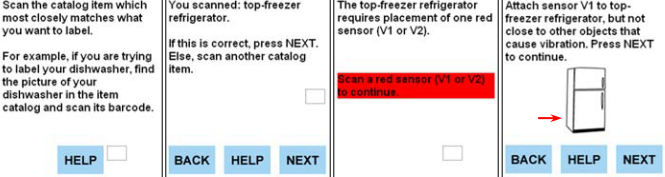
\includegraphics[width=0.8\textwidth]{img/assembly-doku_c.png}
  \caption{Bild des Kits}
  \label{fig:assembly-doku_c}
\end{figure}

Die Installation von Sensoren wird in \cite{Beckmann2004} als eine
Aufgabe mit zwei Dimensionen betrachtet: Platzierung und Assoziation.
Dies sind wichtige Anhaltspunkte um die Randbedinugnen des Modells zu
definieren.


%============================
Expertenwissen wird bei jeder generierung von Dokumentation ben�tigt.
Disadv: AR Handbook not linked to system model

Die Vorteile:
Sehr intuitiv
Automatisch erlernte Dokumentation der Schritte
Unterst�tzung bei der Verifikation der Arbeitsschritte
Passt die Videoausgabe an den Nutzer an

Probleme:
M�ssen wenigstens ein mal Aufgezeichnet werden
F�r Systeme mit vielen Varianten ein potenzielles Problem
�nderung der Prozessschritte zieht ein neues Durchspielen nach sich
Mit Software GUIs nicht ausprobiert
Noch keine Nutzbarkeitsstudie
Expertenwissen wird bei jeder generierung von Dokumentation ben�tigt.
Disadv: AR Handbook not linked to system model

Textuelle Handb�cher genau so gut oder besser?


%% --------------------
%% |   Bibliography   |
%% --------------------
\cleardoublepage
\phantomsection
\addcontentsline{toc}{chapter}{\bibname}

\iflanguage{english}
{\bibliographystyle{IEEEtranSA}}	% english style
{\bibliographystyle{babalpha-fl}}	% german style
												  
% Use IEEEtran for numeric references
%\bibliographystyle{IEEEtranSA})

\bibliography{thesis}


%% ----------------
%% |   Appendix   |
%% ----------------
% \cleardoublepage
% 
% %% appendix.tex
%%

%% ==============================
%\chapter{Appendix}
%\label{ch:Appendix}
%% ==============================

\appendix

\iflanguage{english}
{\addchap{Appendix}}	% english style
{\addchap{Anhang}}	% german style


\section{First Appendix Section}
		\label{Anhang-Implementierung}
		
\setcounter{figure}{0}
		
\begin{figure} [ht]
  \centering
   ein Bild
  \caption{A figure}
  \label{fig:BPMNBeispiela}
\end{figure}


\dots






\end{document}
